% vim: set fenc=utf-8 ft=latex encoding=utf-8
% -*- mode: latex; coding: UTF-8; -*-

\newif\ifdraft
\drafttrue

%%% Marching Triangles.tex

%%%
%%% - ``review'' for content submitted for review
%%% - ``preprint'' for accepted content making available.
%%% - ``tog'' for technical papers accepted to the TOG journal and
%%%	for presentation at the SIGGRAPH or SIGGRAPH Asia conference.
%%% - ``conference'' for final content accepted to a sponsored event
%%% 	(hint: if unsure, use ``conference'') %%% \documentclass[review]{acmsiggraph}

\ifdraft
	\documentclass[conference]{acmsiggraph}
	\def\baselinestrech{1}
	\setlength{\marginparwidth}{2cm}
	\newcommand{\Title}{Investigating Toplogies of Marching Triangles | DRAFT}
\else
	\documentclass[conference]{acmsiggraph}
	\newcommand{\Title}{Investigating Toplogies of Marching Triangles}
\fi


\newcommand{\Author}{Evan T. C. Wilde}
\newcommand{\Email}{etcwilde@uvic.ca}
\newcommand{\Subject}{Using marching triangles algorithm on implicit surfaces}
\newcommand{\Keywords}{iso-surface, polygonization, marching-triangles, blobs}

\synctex=1

\usepackage{xspace}
\usepackage{amssymb}
\usepackage{amsmath}

%% \usepackage[unicode=true,
%% 	bookmarks=false,breaklinks=flase,pdfborder={0 0 0},
%% 	backref=none,colorlinks=false]{hyperref}

\hypersetup{pdftitle={\Title},
	pdfauthor={\Author},
	pdfkeywords={\Keywords},
	pdfsubject={\Subject},
	urlcolor=blue,citecolor=cyan}

\def\BibTeX{{\rm B\kern-.05em{\sc i\kern-.025em b}\kern-.08em
    T\kern-.1667em\lower.7ex\hbox{E}\kern-.125emX}}

\TOGonlineid{V00775033}
\TOGvolume{0}
\TOGnumber{0}

\ifdraft
	\usepackage[colorinlistoftodos]{todonotes}
		\newcommand{\evan}[1]{{\color{cyan}\emph{Evan Says:
		#1}}\xspace}
		\newcommand{\evanTodo}[1]{{\color{blue}\emph{Evan Todo:
		#1}}\xspace}
\else
	\usepackage[disable]{todonotes}
	\newcommand{\evan}[1]{}
	\newcommand{\evanTodo}[1]{}
\fi

\newcommand{\fff}{field falloff function}


%%% Local Variables:
%%% mode: latex
%%% TeX-master: "marching-triangles"
%%% End:


\title{\Title}
\author{
	\Author \\
	University of Victoria\\
	\Email}
\pdfauthor{\Author}
\keywords{\Keywords}

\begin{document}
%%% This is the ``teaser'' command, which puts an figure, centered, below
%%% the title and author information, and above the body of the content.

\teaser{
	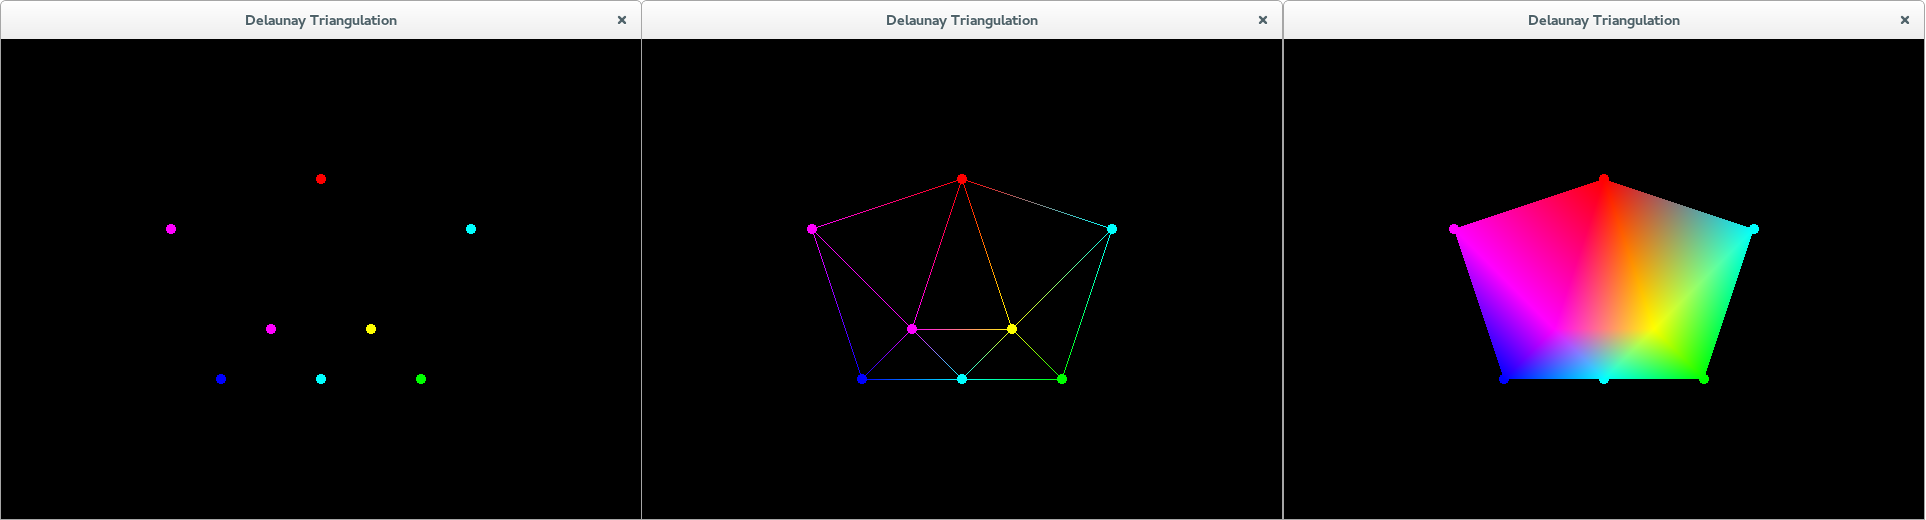
\includegraphics[height=1.5in] {images/Heading.png}
	\caption{Delaunay Triangulation}
}

\maketitle

\begin{abstract}
	Implicit surfaces (iso-surfaces) provide a method to store complex
	geometry. Unfortunately, visualizing implicit surfaces is non-trivial.
	There are two main methods of generating visual representations of
	implicit surfaces, ray tracing and polygonizing. Raytracing creates
	good, accurate image of the surface, however, it takes too long to
	create a representation that is usable in an interactive manner.
	Polygonization is the process of converting an iso-surface to an
	explicitly defined triangle mesh, which can be rendered quickly by the
	computer. Polygonization does not create as accurate visual
	representations, but is able to generate a mesh that is able to be
	rendered in real-time for interactive purposes.

	In this paper, I investigate the range of topologies the Marching
	Triangles algorithm is able to accurately polygonize. I will look at
	the standard cases of simple blobs. Then expand the investigation,
	particularly looking at sharp edges.
\end{abstract}

\keywordlist

\copyrightspace

\section{Introduction}
Implicit surfaces (iso-surfaces) provide a method to store complex geometry or
geometry that cannot be generated in an explicit manner. An iso-surface is
specified with a mathematical formula, and can specify arbitrary geometry. It
is useful in physical simulations and in the games industries. An iso-surface
can contain a massive amount of information, while not requiring as much space.

While iso-surface can maintain accurate details, computers have difficulty
representing them visually. There are two methods for creating a visual
representation of an iso-surface: raytracing or a polygonization algorithm.

Raytracing the surface produces the most accurate visual representation, the
accuracy is only limited by the dimensions of the image being generated, at the
cost of speed. Even with state-of-the-art hardware and the most optimized
raytacing algorithms, raytracers are unable to produce images quickly enough
for interactive real-time rendering of implicit surfaces.

Currently, a popular polygonization algorithm is the Marching Cubes, which
fills the universe with voxels, determines how the surface intersects each
voxel, and results in a plane within the voxel. This results in triangles which
are non-optimal to the topology of the surface, furthermore, there are
ambiguous cases where geometry is lost or cracks emerge. Finally, the marching
cubes algorithm cannot natively handle sharp edges.

An ideal polygonization would meet the following criteria:
it would produce a mesh that does not distort triangles, that is there are no
triangles that are long and narrow; it would produce triangles small enough
that no features of the surface are lost; smooth, flat, surfaces would not be
broken into more triangles than necessary; the mesh should not have holes or
disconnected vertices, and any topology can be converted to a mesh.

The Marching Triangles (MT) algorithm has the potential to create such a
polygonization. The marching triangles is an incremental algorithm that uses
the curvature of the surface to determine where new vertices are placed, either
creating larger triangles where the curvature is small, or creating smaller
triangles where the curvature is large.

In this paper, I investigate the range of geometric topologies the Marching
Triangles algorithm is capable of successfully polygonizing.

\subsection{Introducing implicit surfaces}
This polygonizer works on blobs. A blob is defined as a point in 3D space and a
filter field falloff function, and an iso-value. A common filter field falloff
function is the Metaball function.
\begin{displaymath}
	V(r) = \left\{
		\begin{array}{lr}
			a(1 - {{3r^2}\over{b^2}}) : 0 \le r \le {b\over 3}\\
			{3a\over2}(1 - {r\over b})^2 : {b\over 3} \le r \le b\\
			0 : b \le r
		\end{array}
	\right.
\end{displaymath}

The surface exists where $V(r)$ evaluates to the iso-value.


\section{Related Work}

Research has been performed on converting point-cloud data to triangulations
using a form of the marching triangles algorithm\cite{Scheidegger2005}. This
area is helpful for visualizing the data collected from different sensors
such as, ultrasound pings for robots, LIDAR scans for ocean bathymetry, 3D
scans of objects, or any application where discrete vertices in 3-dimensional
space must be converted to a continuous mesh. The method, also known as the
``Advancing Front algorithm'' builds triangulations of the point cloud using a
3-dimensional generalization of Delaunay triangulation to create a mesh
representation where the triangles are not distorted.

Akkouche presents an implementation of the marching triangles algorithm for
closed implicit surface manifolds\cite{Akkouche2001}. The algorithm provided
topologically correct and geometrically accurate triangle meshes for closed
surfaces. Their results suggest that the marching triangles algorithm runs in
comparable time to the marching cubes algorithm, though the resulting mesh has
higher visual appeal and better overall quality due to the adaptive triangle
size.

Rodrigues de Ara\'{u}jo presents an implementation similar to Marching
triangles. Instead of expanding on edges, it expands on a single
vertex\cite{DeAraujo2004}. This allows them to use Hessian curvature
information instead of approximation methods, providing better results than
traditional marching cubes-based approaches. Furthermore it does not require
computationally heavy re-meshing. \evan{This, Brian, is why I think it will
natively work on sharp edges}

\section{Marching Triangles Algorithm}
The classical marching triangles algorithm begins by creating a seed triangle
on the surface of the object. It adds the three edges to a stack, and begins
iterating. In the iterative step, while the stack is not empty, it pops an
edge, finds a suitable location for a third vertex off of the midpoint of the
selected edge. Then determines if there is an intersection between two
triangles to determine if the fronts are overlapping. If the fronts overlap, it
attempts to merge the two fronts. It returns when there are no more edges on
the front to be processed.

\section {Implementation}

\subsection{Delaunay Triangulation}
The project began with an implementation of Delaunay triangulation to
understand how to get non-distorted triangulations of point-clouds. The
triangulation does not directly apply to the project because I am polygonizing
implicit surfaces, not point clouds. Delaunay triangulation uses voronoi cells
to determine how to triangulate the points in the cloud. For this section, I
will refer to points as elements within the point cloud, and vertices are the
locations where multiple edges of the cells meet. Each vertex is the centre of
a circumcircle defining a triangle. To meet Delaunay, each circumcircle may not
contain a point, and there must be exactly three points on the edge of the
circumcircle. There is an ambiguous case where there are four points arranged
in a perfect square so that no matter how the circumcircles are placed, there
will always be four verticies on the circumcircle. My implementation does not
handle this case.
\begin{figure}
	\centering
	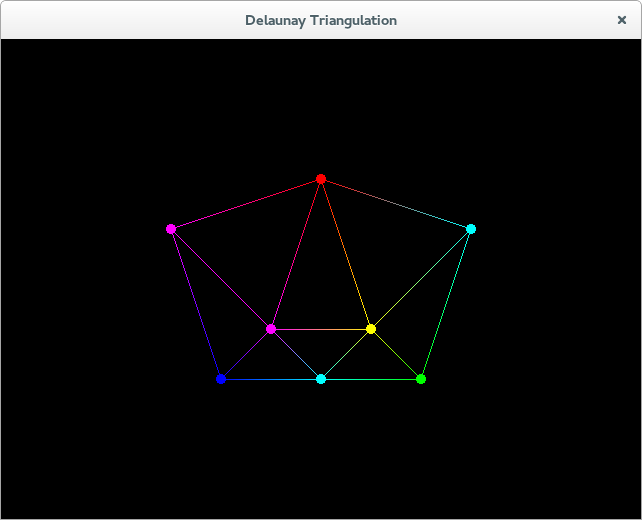
\includegraphics[height=1.5in]{images/Triangulated.png}
	\caption{Delaunay Triangulation}
\end{figure}


\subsection{Implicit System}

The implicit system only uses blobs for now. A blob is defined by a vertex in
3D space and a filter field falloff function. Since we know the centre of the
surface, we can simply use a root finding method to determine where the surface
exists.

I used the secant method, as defined by

$$x_i = x_{i-1} - f(x_{i-1}) \times {{x_{i-1} - x_{i-2}}\over{f(x_{i-1}) -
f(x_{i-2})}}$$

We are able to quickly determine a direction by wiggling\evan{reword this}
the centre vertex to determine in which direction the filter field falloff
function changes most quickly. By multiplying the result of the root-finding
method by the direction vector, we are able to quickly determine where the
iso-surface exists.

The implicit field is defined as follows:
$$\sum\limits_{i=1}^n w_i f(x / \sigma_i ) - T$$
where $w_i$ are weights and $\sigma_i$ are radii and $T$ is the iso-value.

\evan{The stuff beyond here is based off of misunderstandings}
$$f : \mathbb{R}^3 \rightarrow \mathbb{R}$$
$$\rho : A \rightarrow \mathbb{R} $$
$$A = \{x \in \mathbb{R}^3 | f(x) = 0\}$$
$$\phi : \mathbb{R} \rightarrow \mathbb{R}$$

$f$ is the implicit function of the shape. For example, a sphere is defined by
$f(x, y, z) = x^2 + y ^ 2 + z ^ 2 - r^2$ where $r$ is the radius of the sphere.
If the vertex is within the sphere $f(x, y, z) < 0$, when the vertex is on the
surface $f(x, y, z) = 0$, and when the vertex is beyond the sphere $f(x, y, z)
> 0$. If the vertex is not on the surface, we need to map it to the surface.
This operation depends on the surface definition, but will make use of the
gradient to determine which direction the vertex must travel to be on the
surface. An example of a simple projection operation is for the sphere.

$$p_1 = {\nabla f(p_0) \over |\nabla f(p_0)|} \times r$$

$p_0$ defines some initial vertex. $p_1$ is a vertex that lies on the surface
of the sphere.

The sphere is a simple example where the distance from the centre is always the
same and any point on the surface, however it is not necessary for this to be
the case, an example would be a cube. The function $\rho$ converts the vertex
on the surface into a distance, which can be fed into $\phi$, or the field
falloff function.

The end goal is for the vertex to be at some location where the iso-value is
equal to some desired value, for example 0.5.

\subsection{Curvature Information}
Curvature is used in computer graphics to improve meshing of surfaces. Implicit
surfaces are defined by mathematical modles, making it possible to derive the
notion of curvature using differential geometry. There has been research on
methods to determine curvature\cite{DeAraujo2004} of implicit surfaces, however
to my knowledge, they work with a different model of implicit surfaces. The
model used takes $X \in \mathbb{R}^3$ such that $F(X) = 0$, where $F$ is the
implicit function. With this model, shapes are defined algebraically. An
example is a simple sphere where $F(x, y, z) = x^2 + y ^ 2 + z ^2 - R^2$. This
model lends itself nicely to determining gradients. The gradient is defined as
follows: $\overrightarrow{G} = \nabla F(X) = [{\partial F\over\partial x},
{\partial F \over \partial y}, {\partial F \over \partial z}]$ and the normal
$\overrightarrow{N} = {\overrightarrow{G} \over ||\overrightarrow{G}||}$.

We can determine the gradient\cite{Stam2011} with a method.



\section{Results}
No results yet\ldots.

\subsection{Issues with the Implicit Model}
The model used for defining implicit surfaces does not lend itself nicely to
determining gradient vectors. It requires samples along the $x$, $-x$, $y$,
$-y$, $z$ and $-z$ axes. Along each axis, we must project the vertex onto
the surface and determine which direction has the greatest change. Due to this
model, we must sample the implicit surface more to determine the gradient,
hurting performance.

\evanTodo{Find results!}

\section{Conclusions and Future Work}


\bibliographystyle{acmsiggraph}
\bibliography{references}



\end{document}

